% % % % % % % % % % % % % % % % % % % % % % % % % % % % % % % % % % % %
%\documentclass[english]{article}
\documentclass{acm_proc_article-sp}
%\usepackage[T1]{fontenc}
\usepackage[latin9]{inputenc}
%\usepackage{fancyhdr}
%\pagestyle{fancy}
%\usepackage{textcomp}
%\usepackage{babel}
\usepackage{url}
\usepackage{color,soul}
\usepackage{graphicx}
\usepackage[pdftitle={Adaptive Geo--Replication Based on Ant Colony Algorithm},%
		hidelinks,colorlinks=true, linkcolor=black, citecolor=cyan, filecolor=green, urlcolor=blue]{hyperref}
\usepackage{mathtools}
\usepackage{amssymb}
\usepackage[numbers]{natbib}
%\usepackage{glossaries}
%\usepackage[xindy]{glossaries}

\usepackage{multirow}
\usepackage{rotating}

%\makeglossaries

% % % % % % % % % % % % % % % % % % % % % % % % % %
% Aconyms for SyncFree project.
%
% Author: Amadeo Asco
% Last updated: 24 July 2014
% % % % % % % % % % % % % % % % % % % % % % % % % %
% The acronym package helps you manage acronyms and acronym lists in your documents, http://www.mackichan.com/index.html?techtalk/456.htm~mainFrame
% for the glossary to show up in Table of Contents you need to additionally add toc option
\usepackage[toc,nonumberlist]{glossaries}
%\showthe\hsize% interrupts latex and shows value of \hsize
\setlength{\glsdescwidth}{0.82\hsize}%
% to remove extra line between groups
\renewcommand{\glsgroupskip}{}
% To get rid of the full stop after the description in the glossary
\renewcommand{\glspostdescription}{}
\makeglossaries

% Start definitions ---------------------------
% Add all of the definitions for the abbreviations
\newacronym{2i}{2i}{Secondary Indexing}
\newacronym{2pset}{2P-Set}{Two-Phase Set}
\newacronym{acid}{ACID}{Atomicity, Consistency, Isolation, Durability}
\newacronym{b2b}{B2B}{Business to Business}
\newacronym{base}{BASE}{basically available, soft state, eventual consistency}
\newacronym{cci}{CCI}{Causality, Convergence and Intention}
\newacronym{cmrdt}{CmRDT}{Op-based Convergent Replicated Data Type}
\newacronym{cprdt}{CPRDT}{Conflict-free Partially Replicated Data Type}
\newacronym{crdt}{CRDT}{Conflict-free Replicated Data Type}
\newacronym{cqrs}{CQRS}{Command Query Responsibility Segregation}
\newacronym{cvrdt}{CvRDT}{State-based Convergent Replicated Data Type}
\newacronym{dc}{DC}{Data Centre}
\newacronym{ec}{EC}{Eventual Consistency}
\newacronym{ga}{GA}{Genetic Algorithm}
\newacronym{gset}{G-set}{State-based increment-only Counter}
\newacronym{gp}{GP}{General Practitioner}
\newacronym{ha}{HA}{High Availability}
\newacronym{id}{ID}{identifier}
\newacronym{lww}{LWW}{Last-Writer-Wins}
\newacronym{lwwr}{LWW-Register}{Last-Writer-Wins Register}
\newacronym{mdc}{MDC}{Multi Data Centre}
\newacronym{mv}{MV}{Multi-Valued}
\newacronym{mvr}{MV-Register}{Multi-Valued Register}
\newacronym{orset}{OR-set}{Observed-Removed Set}
\newacronym{rdbms}{RDBMS}{Relational Database Management System}
\newacronym{rga}{RGA}{Replicated Growing Array}
\newacronym{rest}{REST}{Representational State Transfer}
\newacronym{rpc}{RPC}{Remote Procedure Call}
\newacronym{cap}{CAP}{Consistency, Availability and Partition tolerance}
\newacronym{sec}{SEC}{Strong Eventual Consistency}
\newacronym{ttl}{TTL}{Time To Live}
\newacronym{uset}{U-Set}{Two-Phase Set with unique elements}
\newacronym{wp1}{WP1}{Work Package 1}
\newacronym{wp2}{WP2}{Work Package 2}
\newacronym{wp3}{WP3}{Work Package 3}
\newacronym{wp4}{WP4}{Work Package 4}
\newacronym{wp5}{WP5}{Work Package 5}
% end abbreviations ---------------------------

%\ifnum\showDefinitions=1
% Add all of the definitions
%\newglossaryentry{bwd}{name={box-and-whisker diagram}, text={box-and-whisker diagram}, first={box-and-whisker diagram},
%    description={\parbox{10.6cm}{\medskip The bottom and top of the box are the 25th and 75th percentile (the lower and upper quartiles, respectively), and the band near the middle of the box is the median, whereas the dot represent the mean. The ends of the whiskers represent the minimum and maximum of all of the data.\medskip}}}
% end definitions -----------------------------
%\fi

\glsdisablehyper


\begin{document}

\title{Adaptive Geo--Replication Strategy}

\author{Amadeo Asc\'{o}\\ Trifork Leeds, Leeds, UK}

\date{24$^{th}$ September 2014}

\maketitle

\abstract
The amount of data being processed in \glspl{dc} keeps growing at enormous rate so that full replication may start being impractical. The use of replication between \glspl{dc} is used to increase data availability in the presence of site failures and to reduce access costs by accessing the data locally, if possible. This means that replicating the data only in some of the \glspl{dc} is becoming more critical to reduce the costs of keeping the data consistent or eventually consistent and still maintaining a high availability (scalability) and low access costs. For changing patterns of read and write data requests the data to be replicated and the its location has to be obtained dynamically. Given that the problem of finding an optimal replication schema in a general network has been shown to be NP-complete for the static case, it is unlikely to be able to generate a general algorithm to find efficient solutions to the dynamic problem.

So a new adaptive bio-inspired replication strategy is presented here, which is completely decentralised, adaptive, inspired on the Ant Colony algorithm, and event-driven. Also the replication protocol is independent of the strategy implemented but it is guided by the strategy.\\

\keywords
Adaptive Replication, Geo-replication, Multiple \glspl{dc}, Large-Scale Database Replication, Partial Replication, Scalability


\section{Introduction}
	The amount of data being processed in \glspl{dc} keeps growing at enormous rate \cite{Tolle2011a, Cisco2014a, Chanthadavong2014a}. Some of the areas where the amount of stored data already reach \glspl{tb} and even \glspl{pb} are data mining, particle physics, climate modelling, high energy physics and astrophysics, to site few, data which needs to be shared and analysed \cite{KingsyGrace2013a, MohdZin2012a, Naseera2009a}. \glspl{dc} are able to ensure that stored data is highly accessible and scalable. But the location of a \gls{dc} in respect of the client accessing the data has an impact on availability, access times (latency - accessibility) and costs derived from providing the data. Replicating some of the data at multiple sites is a possible solution to reduce some of these undesirable effects, \cite{Briquemont2014a, Abad2011a, Venugopal2006a}. An increase in the number of replications may result in a large bandwidth savings and lead to a reduction in user response time on reads or writes depending on the replication type, i.e. replication on read or write. But keeping too many replicas of the data incurs in extra costs, such as extra replication traffic to keep all versions of the data coherent, extra required storage and extra computational power \cite{Serrano2007a, Goel2006a}.
	
	This means that finding an optimal replication distribution that minimises the amount of network traffic given certain read and write frequencies for various objects should alleviate these extra costs when replicating, \cite{Wolfson1990a, Briquemont2014a}. Given the volume of operations considered, which are predominately higher in reads than writes, and the speed of the access expected then any algorithm suitable to be applied to this constrain optimisation problem must have a very fast execution time or it will have a detrimental effect in the latency.

	The replications may be grouped, base on its existence, into two types; {\bf static replication} where a replica persist until it is deleted by a user or its duration expires, and {\bf dynamic replication} where the creation and deletion of a replica are managed automatically and normally directed by the access pattern of the data used by the users \cite{Dong2008a}. In static replication the major drawback is their inability to adapt to changes in the access pattern of the data used by the users.
	
	Also there are two types of replication based on their effect on the data; {\bf partial replication} is concerned in the number of parts the full data is composed, all of which may be located in different parts of the overall system, i.e. \glspl{dc}, within a \gls{dc} in different nodes or at the client-side \cite{Briquemont2015a, Briquemont2014a, Serrano2007a}, whereas {\bf adaptive geo--replication} is concerned in what data and where the data or part of the data is located within the overall system of \glspl{dc} and how many replicas exist simultaneously, \cite{KingsyGrace2013a, Wang2012a, Abad2011a, Abdul-Wahid2007a, Loukopoulos2004a}.
	
	The problem of finding an optimal geo--replication schema in a general network has been shown to be NP-complete for the static case \cite{Apers1988a,Wolfson1997a,Wolfson1991a} so there is no known efficient geo--replication algorithm to locate a convergent optimal solution dynamically. Given this it is proposed an algorithm base on Wolfson's algorithm, \cite{Wolfson1990a}, which proposes an adaptive algorithm for replicated data between processors which takes into account the changes in the read-write pattern of the processors in the network, and it is also based on the principles of the Ant Colony Optimisation algorithms, which are inspired in the behaviour of ant colonies when deciding which path to follow when foraging, \cite{dorigo1992a}.%cite{jeanson2003}
	
	It should be noted that the main propose of the replication is not to recover from disasters as this is the responsibility of the recovery centres which are data centres sufficiently close to the operational \gls{dc}, they are associated to, so copies can be processed quickly enough but at the same time sufficiently far apart as to avoid any potential geographical issues that may happen to the \glspl{dc}, i.e. earthquakes, fire that destroys the \gls{dc}, the shutting down of main power plant which provides energy to the \gls{dc}. Neither it is the \gls{dc} responsibility to provide analytical services as these are provided by the data warehouse(s). The main propose of the considered \glspl{dc} is to provide operational access to clients (operational \glspl{dc}), which corresponds to intensive read/write operations to the client's most recent data. The following references to \glspl{dc} in this document referrer to operational data centres.


\section{Algorithm}
The general idea of this algorithm is to decide without the need of human intervention where and when to replicate with the main objective of reducing the latency and network traffic (reduce usage of bandwidth).

In general terms any read operation in a \gls{dc} reinforces the need for a replica of the data in such \gls{dc}, similarly but perhaps with a different degree it happens with the write operations, but write operations decrease the need for a replica of the data in the other \glspl{dc} with replicas of the data, so eventually these \glspl{dc} will not have any replica of the data. Given that we do not want to keep replicas if it is not necessary then the need for such replica will decay as time pass, but always making sure that the data is present (replicated) at least in one of the \glspl{dc}. This algorithm is further explained below together with a mathematical representation. The variables and constants used in the algorithm are summarised in Table \ref{tbl:vars_consts}.
\begin{table*}[ht!]
	\begin{tabular}{ |l|p{13.5cm}|l|}
		\hline
		{\bf Variable}    & {\bf Description} & {\bf Type} \\
		\hline
		\hline
		$DC$                & It is the set of all \glspl{dc}. $d$ identifies one of the \glspl{dc}, $d \in \{1,\dots, |DC|\}$. \gls{dc}$_{d}$ represents the \gls{dc} $d$ which holds some data, D$_{d}$. &  $d \in \mathbb{N}^{+}$ \\
		\hline
		$D_{kd}$           & It represents the replica of data $k$ in \gls{dc} $d$, $k \in \{1,\dots, |D|\}$. & $k \in \mathbb{N}^{+}$ \\
		\hline
		$r_{kd}$            & It is the number of reads for data $k$ requested on \gls{dc} $d$. & $r_{kd} \in \mathbb{N}_{0}$ \\
		\hline
		$\Delta r_{k}$   & It represents the strengthening of the replication in the \gls{dc} used to execute one read. & $\Delta r_{k} \in \mathbb{R}^{+}$ \\
		\hline
		$w_{kd}$           & It is the number of writes for data $k$ directly requested on \gls{dc} $d$. & $w_{kd}\in \mathbb{N}_{0}$ \\
		\hline
		$\Delta w_{k}$  & It represents the strengthening of the replication in the \gls{dc} directly used to execute a write. & $\Delta w_{k} \in \mathbb{R}^{+}$ \\
		\hline
		$w_{kdi}$          & It represents the decay of the replication in the \gls{dc} $i$ consequence of the write request in \gls{dc} $d$. This value will depend of both \glspl{dc} $d$ and $i$ and may also depend on the time of the day or other useful information available at the time it is used. & $w_{kdi} \in \mathbb{R}^{+}$ \\
		\hline
		$\Gamma$      & It is the decay of the replication strength with time. A simple example corresponds to a constant decay ($\tau$) of the replication strength from the time the replica was created, $\Gamma = \Delta t * \tau$. & $\Gamma \in \mathbb{R}^{+}$ \\
		\hline
		$N_{k}$           & Minimum number of replicas of data k with $1 \le N_{k} \le |DC|$, default $N_{k} = 1$. The number of \glspl{dc} that can be safely removed from the system without information loss is $N_{k} -1$. & $N_{k} \in \mathbb{N}^{+}$ \\
		\hline
		$T^{+}_{k}$       & It is the replication strength required to start the replication of data $k$ in a \gls{dc} which does not currently contain a replica of the data. & $T^{-}_{k} \in \mathbb{R}^{+}$ \\
		\hline
		$T^{-}_{k}$       & It is the replication strength from where the replication of the data is removed $k$ in a \gls{dc} which contains currently a replica of the data, default $T^{-}_{k} = 0$. & $T^{-}_{k} \in \mathbb{R}^{+}$ \\
		\hline
		$L_{k}$            & The maximum replication strength for data $k$. & $L_{k} \in \mathbb{R}^{+}$ \\
		\hline
		$F_{k}$            & The replication strength for data $k$, $F_{k} \le L_{k}$. & $F_{k} \in \mathbb{R}^{0}$ \\
		\hline
		$R_{k}$            & It is the number of replicas for data $k$, $D_{k}$, with $1 \le N_{k} \le R_{k} \le |DC|$. & $R_{k} \in \mathbb{N}^{+}$ \\
		\hline
		$X_{kd}$            & It refers to the existence of a replica of data $k$ in \gls{dc} $d$, with value $1$ if the replicas exists or $0$ otherwise. & $X_{kd} \in (0, 1)$\\
		\hline
	\end{tabular}
	
	\caption{List of variables and constants.}
	\label{tbl:vars_consts}
\end{table*}

Equation \ref{eq:data_replicated} represents the existence of a replica of data $k$ in \gls{dc} $d$, $X_{dk} = 1$, or its absence $X_{dk} = 0$. $R_{k}$ is the number of replicas of data $k$, as expressed in Equation \ref{eq:num_replicas}.
\begin{equation} \label{eq:data_replicated}
	X_{kd} = \left\{
		\begin{array}{ll}
			1 & if D_{k} \in DC_{d} \text{ } (\exists D_{kd})\\
			0 & otherwise
		\end{array}
	\right.
\end{equation}

\begin{equation} \label{eq:num_replicas}
R_{k} = \sum^{|DC|}_{d = 1} X_{dk}
\end{equation}

$F_{kd}$ represents the full strength of the replication of the data $k$ in \gls{dc} $d$, which it is expressed in Equation \ref{eq:replication_strength}.
\begin{equation}  \label{eq:replication_strength}
	\begin{split}
		 F_{kd} = \max(0, \min(L_{k}, r_{kd} * \Delta r_{k} + w_{kd} * \Delta w_{k}\\
		 - \sum^{|DC|}_{i = 1, i \neq d} w_{kd} * \Delta w_{kdi} - X_{kd} * \Gamma))
	 \end{split}
\end{equation}

%\begin{equation}  \label{eq:inter_dc_decay}
%	\Delta w_{kdi} = 0 \textbf{ } \forall d = i \text{ or } X_{kd} = 0 \text{, or } X_{ki} = 0
%\end{equation}

Equation \ref{eq:replication_strength} shows that the replication strength for the data $k$ in \gls{dc} $d$ is strengthened by the reads and writes requested through \gls{dc} $d$, with intensities $\Delta r_{k}$ and $\Delta w_{k}$ respectively, and weakened  by the writes requested through other \glspl{dc} than \gls{dc} $d$, with intensity $\Delta w_{kdi}$, and it is furthermore weakened by a temporal decay on the replication strength (last term in the equation). Where Equation \ref{eq:replication_strength} states that only \glspl{dc} with a replica of the data, $D_{k}$, will be penalised by writes and time, which in practice it is achieved by not sending the write to those \glspl{dc} so it does not incurred in any extra cost when implementing it. Similarly $\Gamma$ will not be applied to \glspl{dc} without replicas of the data with the exceptions of those candidate \glspl{dc} where the data may later be replicated. Reads may increase the number of replicas where writes may strengthen the replication in a \gls{dc} but may also potentially remove a replica from one of the other \glspl{dc}, effect that it is strengthen by the temporal decay of the replication strength.

$T^{+}_{k}$ is the threshold of the replication strength of data $k$ which determines when to keep an existing replica in a \gls{dc}, as expressed in Equation \ref{eq:replicas_threshold+}.
\begin{equation} \label{eq:replicas_threshold+}
	\begin{split}
		F_{kd} \le T^{+}_{k} \text{, } \nexists D_{kd} \text{, } t < t_{0}  \wedge F_{kd} > T^{+}_{k} \text{, } t_{0} \Longrightarrow \exists D_{kd} \text{, }\\
		 t_{0} \text{ } (D_{kd} \in DC_{d})
	\end{split}
\end{equation}

$T^{-}_{k}$ is the threshold of the replication strength of data $k$ which determines when to remove an existing replica in a \gls{dc} when the other constrains are still kept. i.e. minimum number of replicas, as expressed in Equation \ref{eq:replicas_threshold--}. Also a simple view of the thresholds is shown in Figure \ref{fig:lim_constriants}.
\begin{equation} \label{eq:replicas_threshold--}
	\begin{split}
		F_{kd} > T^{-}_{k} \wedge \exists D_{kd} \text{, } t < t_{0}  \wedge F_{kd} \le T^{-}_{k} \text{, } t_{0} \Longrightarrow \nexists D_{kd} \text{, }\\
		 t_{0} \text{ } (D_{kd} \in DC_{d})
	\end{split}
\end{equation}
\begin{center}
	\begin{figure}[ht!]
		\centering
		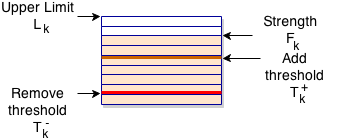
\includegraphics[width=.51\textwidth]{figures/strengthReplica.png}
	
		\caption{Constraints.}
		\label{fig:lim_constriants}
	\end{figure}
\end{center}

The Equations \ref{eq:no_replica} and \ref{eq:replicas_threshold} show the cases where a data $k$ is not replicated in a \gls{dc} $d$.  A replica in a \gls{dc}, with a replication strength not bigger than the reduction replication strength ,$T^{-}_{k}$, will only be destroyed if the number of replicas is bigger than a minimum, $N_{k}$, as represented in Equation \ref{eq:no_replica}. Also for a \gls{dc} which does not have a replica of the data the replication strength must be higher than a pre-set threshold $T^{+}_{k}$ to create a new replica, as represented in Equation \ref{eq:replicas_threshold}.
\begin{equation} \label{eq:no_replica}
	\exists D_{kd} \text{, } t < t_{0} \text{, } R_{k} > N_{k} \text{, } F_{kd} > T^{-}_{k} \Longrightarrow \nexists D_{kd} \text{, } t_{0} \text{, } F_{kd} \le T^{-}_{k}
\end{equation}

\begin{equation} \label{eq:replicas_threshold}
	\nexists D_{kd} \text{, } t < t_{0} \text{, } F_{kd} \le T^{+}_{k} \Longrightarrow \nexists D_{kd} \text{, } t_{0} \text{, } F_{kd} \le T^{+}_{k}
\end{equation}

Each \gls{dc} with a replica of the data must know about the other \glspl{dc} that have replicas of the same data in order to manage the replication of such data.

If data $k$ is only replicated in one \gls{dc} $d$ and a write is requested using a different \gls{dc} $j$ than the one it is currently replicated in, so that its replication strength in \gls{dc} $d$ is reduced to zero or under ($F_{kd} < 0$), then the data will continue to be replicated in that \gls{dc} until a replica is place in another \gls{dc} or its replication is increased over zero.

For the time being, it is considered the case where $w_{kdi}$ increases with the distance (network distance) between both \glspl{dc} $d$ and $i$. Also it is assumed that the value is symmetrical, such that $w_{kdi} = w_{kid}$, so there is the same cost of transferring the data from \gls{dc} $d$ to \gls{dc} $i$ than from \gls{dc} $i$ to \gls{dc} $d$. If to transfer the data between both \glspl{dc} $d$ and $i$ requires the use of an intermediate \gls{dc} $j$ then $w_{kdi} \ge w_{kdj} + w_{kji}$, similarly if many intermediate nodes are used the decay will be at least the sum of the intermediate decays.

The effect of $\Gamma$ is required to ensure that in absence of writes some replications will still vanish and if the reads are concentrated in a few \glspl{dc} then the replicas in other \glspl{dc} will be eventually removed. There is an extra requirement in the case that the data only exists in a \gls{dc}, in which case, the temporal effect should be ignored, so the data exists at least in one \gls{dc}.

A read request to a \gls{dc}, which does not have a replica of the data, will be forwarded to the closest \gls{dc} with a replica. The \gls{dc} with a replica will not gain strength from this read operation as the read was not initiated directly from itself. This \gls{dc} will then have a knowledge of the data but not a replica, so this knowledge will be used in subsequent reads/writes to the \gls{dc} which eventually may keep a replica. Once the replication strength is higher than the threshold ($T^{+}_{k}$), this \gls{dc} will notify all the \glspl{dc} with a replica of the existence of the new \gls{dc} with a replica.

It may also be required to use another temporal effect, the \gls{ttl}, to make sure that eventually the data will be fully removed. This value may not be applied to data stored in recovery centres and data warehouses which may have their own \gls{ttl}. Also it would be desirable for data that expires to be copied into those data centres before it is removed from all the \glspl{dc}.

Overall it is assumed that reads and writes are not treated differently (not using \gls{cqrs}), so they are not directed to different \glspl{dc}, otherwise it may be needed some adjustment to the approach presented here or may even invalidate it.

The algorithm is optimal in the sense that when the replication scheme stabilises, the total number of replicas required for the reads and writes is minimal.

The read sequence diagrams for this algorithm are shown in Table \ref{tb:read_sequence_diagrams} with its flowchart presented in Figure \ref{fig:read_flowchart}, and the write ones are shown in Table \ref{tb:write_sequence_diagrams} with its flowchart presented in Figure \ref{fig:write_flowchart}. The second figure in Table \ref{tb:read_sequence_diagrams} may also have a notification for all \glspl{dc} with a replica of the data to notify of the new replica which will be sent by the direct \gls{dc} for when the threshold has been passed and a replica is created in the direct \gls{dc}.
\begin{table}[ht!]
	\begin{center}
		\begin{tabular}{c}
			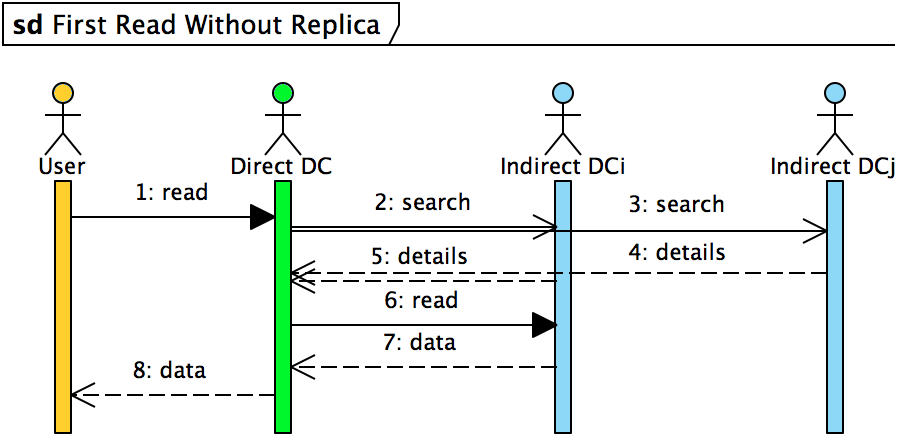
\includegraphics[width=.48\textwidth]{figures/firstReadWithoutReplica.png} \\
			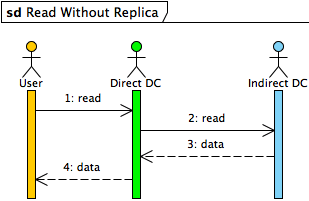
\includegraphics[width=.35\textwidth]{figures/readWithoutReplica.png} \\
			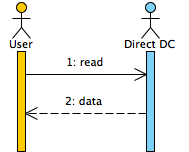
\includegraphics[width=.23\textwidth]{figures/readWithReplica.png}
		\end{tabular}
		
		\caption{Read Sequence Diagrams on write replication.}
		\label{tb:read_sequence_diagrams}
	\end{center}
\end{table}
\begin{figure}[ht!]
	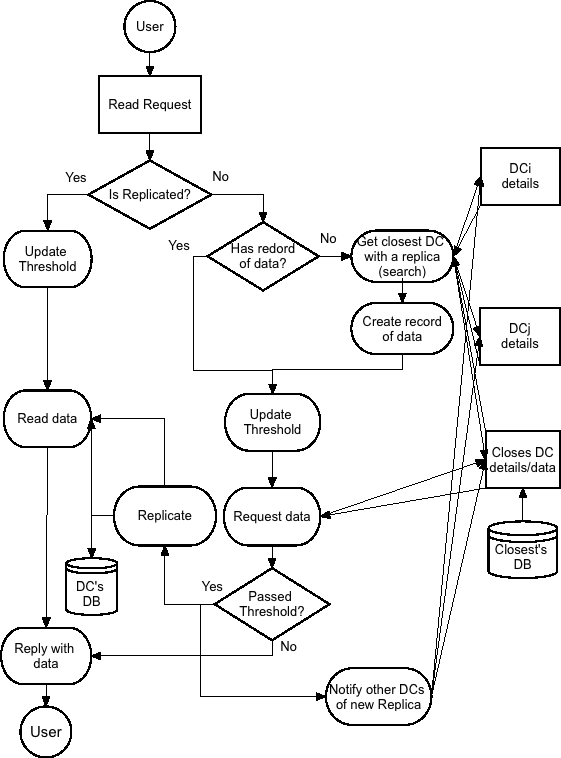
\includegraphics[width=.47\textwidth]{figures/readRequestFlowchart.png}

	\caption{Flowchart for read requests.}
	\label{fig:read_flowchart}
\end{figure}
\begin{table}[ht!]
	\begin{center}
		\begin{tabular}{c}
			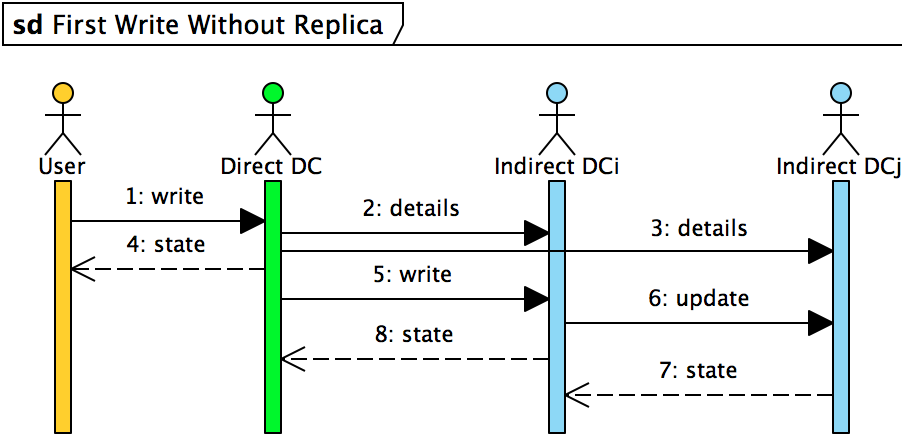
\includegraphics[width=.46\textwidth]{figures/firstWriteWithoutReplica.png} \\
			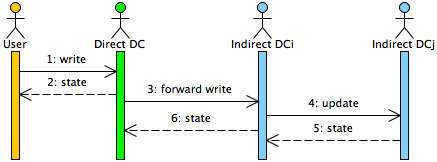
\includegraphics[width=.47\textwidth]{figures/writeWithoutReplica.png} \\
			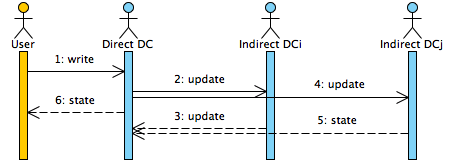
\includegraphics[width=.47\textwidth]{figures/writeWithReplica.png}
		\end{tabular}
		
		\caption{Write Sequence Diagrams on write replication.}
		\label{tb:write_sequence_diagrams}
	\end{center}
\end{table}
\begin{figure}[ht!]
	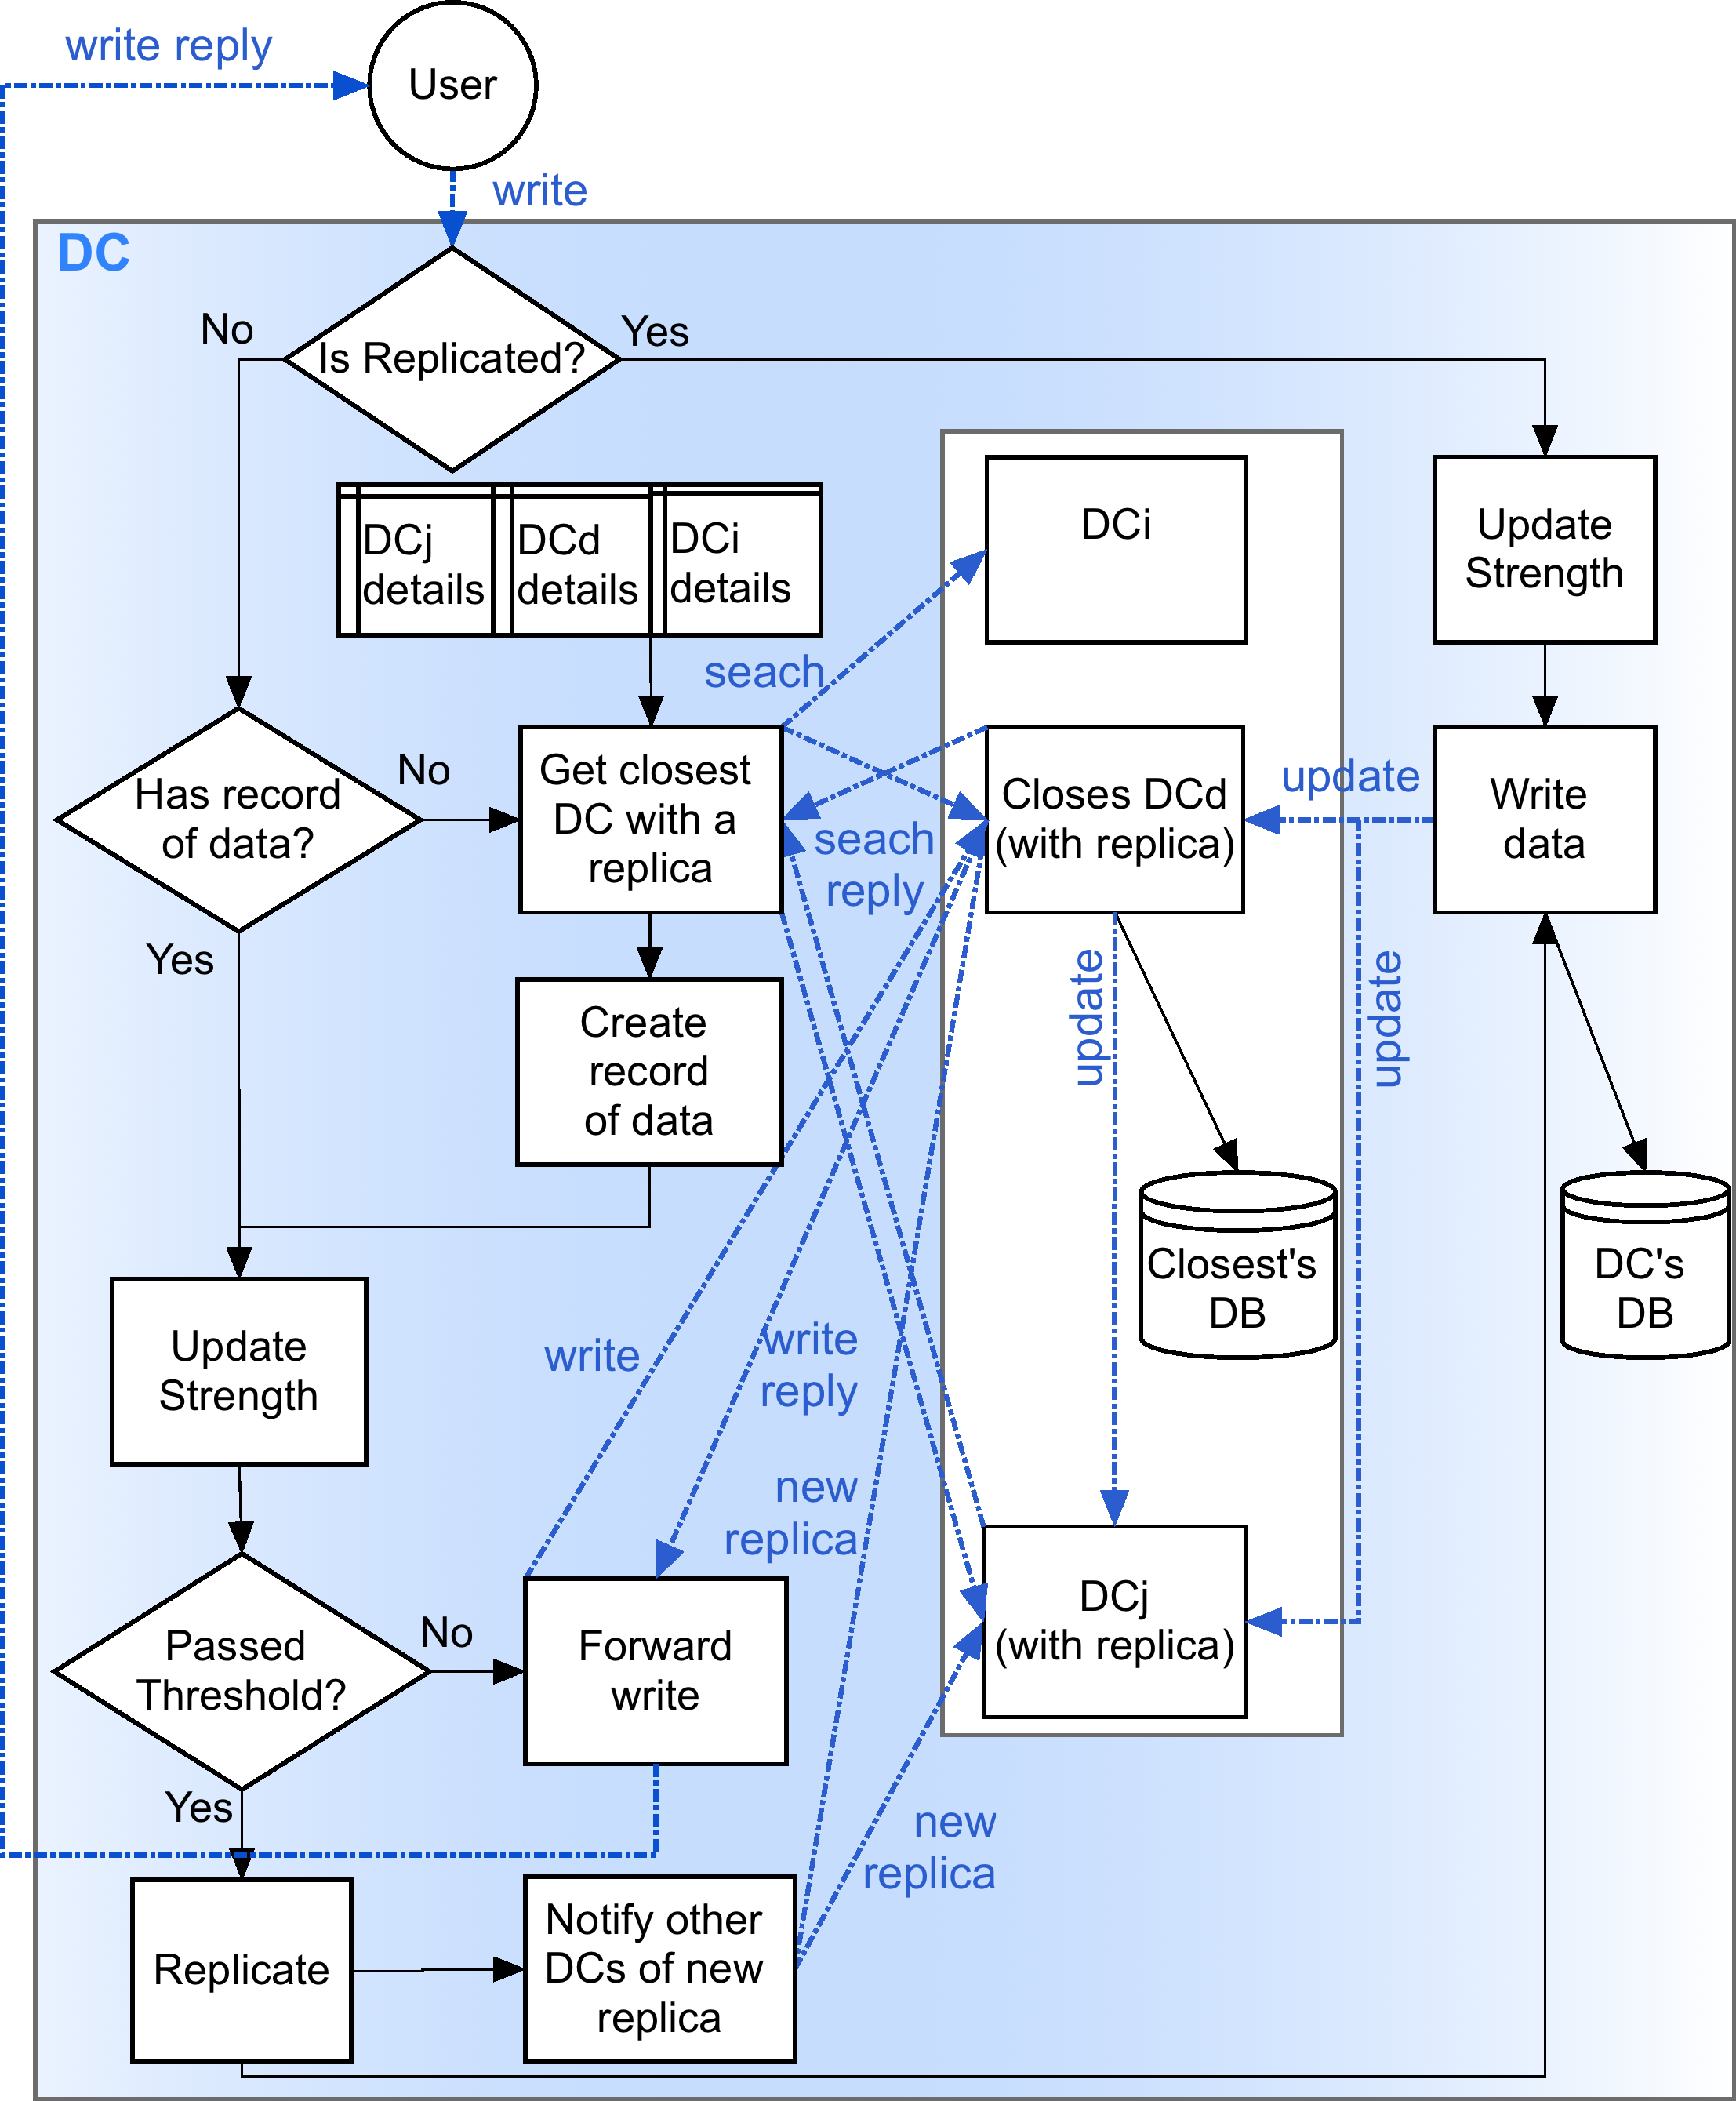
\includegraphics[width=.47\textwidth]{figures/writeRequestFlowchart.png}
	
	\caption{Flowchart for write requests.}
	\label{fig:write_flowchart}
\end{figure}

The creation of data will generate a replica in the directly accessed \gls{dc}, as the number of replicas must be at least one ($M_{k} \ge 1$). If the minimum number of replicas is bigger than 1 then the algorithm should generate and distribute the other replicas between the vicinity \glspl{dc}. It is proposed that the approach distributes the created replicas to be implemented as a pluggable distribution approach, i.e. distribute replicas within the vicinity. The creation of the data will require to check if the data exists already, i.e. in a key value tuple that the key does not al;ready exist in any of the other \glspl{dc}. Then only in the case where the data does not already exist in any of the \glspl{dc} the data will be replicated in the direct accessed \gls{dc} and distributed replicas within other of the \glspl{dc} based on the current creation approach and the minimum number of replicas.


{\bf Some notes on parameters}: 

Given that the number of read is expected to be higher than the number of writes, and normally a read will be executed before a write, it may make sense for $\Delta w_{k}$ to be smaller than $\Delta r_{k}$ ($\Delta w_{k} < \Delta r_{k}$) so that more writes would be required to maintain or create a replica in a \gls{dc} than when using reads.

Some of the parameters may be generalised even further by allowing them to depend on the \gls{dc} the calculation executed in, e.g. $\Delta r_{kd}$ instead of $\Delta r_{k}$ and $\Delta w_{kd}$ instead of $\Delta w_{k}$. Even the terms $r_{k} * \Delta r_{k}$ and $w_{k} * \Delta w_{k}$ could be generalise to consider other factors like bandwidth used and current storage capacity available in the \gls{dc}, or new terms could be added to take account of those new factors.

\citet{Paiva2013a} use a very simple representation of the available storage capacity, which is taking into account in the replication of the data. We have assumed that the capacity in a \gls{dc} is sufficient and when more storage capacity is required then extra storage is added to the \gls{dc}. If this is not the case and $S^{d}$ is the total storage capacity in \gls{dc} $d$, and $S_{k}$ is the size of the data to store then Equation \ref{eq:free_storage} provides the free storage available in \gls{dc} $d$, $s^{d}$.
\begin{equation} \label{eq:free_storage}
	s^{d} = S^{d} - \sum^{|D|}_{k = 1} S_{k} * X_{kd}
\end{equation}

Accessibility in general is increased for Adaptive replication when compared to no replication. But also accessibility in general decreases for Adaptive replication when compared to full replication, given that when less replicas exit there is more chances that, on partition, a user is in the side of the partition where there is not any replica. Of course, this can be reduced by increasing the minimum number of replicas that must exist at each time and even adding extra constraints in relation to where those replicas must be in relation to each other.


\subsection{Mathematical Cost Representation} \label{sec:math_cost_representation}
It is considered that there is a direct cost associated to the reads ($c^{r}_{kd}$) and writes ($c^{w}_{kd}$) executed in the system for the data $k$ in the \gls{dc} $d$. Also there is a cost associate to the reads ($c^{r}_{kdj}$, $c^{r}_{kdd} = 0$) and writes ($c^{w}_{kdj}$, $c^{w}_{kdd} = 0$) between \glspl{dc} $d$ and $j$ for data $k$, shown in Table \ref{tb:costs}.
\begin{table*}[ht!]
	\begin{center}
		\begin{tabular}{|l|p{13.6cm}|l|}
			\hline
			Cost                         & Description & Type \\
			\hline
			\hline
			$X_{kd}(t)$            & It refers to the existence of a replica of data $k$ in \gls{dc} $d$ for time $t$, with value $1$ if the replicas exists or $0$ otherwise. & $\{0, 1\}$\\
			\hline
			$r_{kd}(t, t+dt)$       & It is the number of reads for data $k$ requested on \gls{dc} $d$ from time $t$ to $t+dt$. It could be also represented as $r_{kd}(t, t+dt) = r_{kd}(t+dt) - r_{kd}(t)$, where $r_{kd}(t)$ is the number of reads from the beginning up to time $t$. & $\mathbb{N}_{0}$ \\
			\hline
			$w_{kd}(t, t+dt)$      & It is the number of writes for data $k$ directly requested on \gls{dc} $d$ from time $t$ to $t+dt$. It could be also represented as $w_{kd}(t, t+dt) = w_{kd}(t+dt) - w_{kd}(t)$, where $w_{kd}(t)$ is the number of writes from the beginning up to time $t$. & $\mathbb{N}_{0}$ \\
			\hline
			$\rho_{kd}(t, t+dt) $ & The existence of an operation from time $t$ to $t+dt$, witch is 1 if $(r(t, t+dt)_{kd} + w(t, t+dt)_{kd}) > 0$ or zero otherwise. & $\{0, 1\}$ \\
			\hline
			$c^{r}_{kd}(t)$           & The cost of a read request of the data $k$ to \gls{dc} $d$ for time $t$. & $\mathbb{R}^{+}$ \\
			\hline
			$c^{w}_{kd}(t)$          & The cost of a write request of the data $k$ to \gls{dc} $d$ for time $t$. & $\mathbb{R}^{+}$ \\
			\hline
			$c^{r}_{kdj}(t)$           & The cost of a read request of data $k$ from \gls{dc} $d$ to \gls{dc} $j$, and $c^{r}_{kdd} = 0$ for time $t$. & $\mathbb{R}^{+}$ \\
			\hline
			$c^{r}_{*dj}(t)$           & The cost of a search request from \gls{dc} $d$ to \gls{dc} $j$, and $c^{r}_{*dd} = 0$ for time $t$. & $\mathbb{R}^{+}$ \\
			\hline
			$c^{w}_{kdj}(t)$         & The cost of a read request of data $k$ from \gls{dc} $d$ to \gls{dc} $j$, and $c^{w}_{kdd} = 0$ for time $t$. & $\mathbb{R}^{+}$ \\
			\hline
		\end{tabular}
	\end{center}

	\caption{Costs and variables time dependent.}
	\label{tb:costs}
\end{table*}

The cost between time $t$ and $t+dt$ is expressed by Equation \ref{eq:cost_operations} and the minimum number of replicas is represented by Inequality \ref{ineq:limit_replicas} for time $t$.
\begin{equation} \label{eq:cost_operations}
	\begin{split}
		 Cost_{k}(t, t+dt) =\\
		  \sum^{|DC|}_{d = 1} \left(\underbrace{r_{kd}(t, t+dt) * c^{r}_{kd}(t) + w_{kd}(t, t+dt) * c^{w}_{kd}(t)}_\text{direct cost} \right. \\
		 \left. + \underbrace{\sum^{|DC|}_{j = 1} w_{kd}(t, t+dt) * c^{w}_{kdj}(t) * X_{kj}(t)}_\text{update propagation cost} \right. \\ 
		 \left. + \underbrace{(1 - X_{kd}(t)) * r_{kd}(t, t+dt) * \min_{j \in R_{k}}(c^{r}_{kdj}(t))}_\text{redirect reads cost} \right. \\  
		 \left. + \underbrace{(1 - X_{kd}(t)) * w_{kd}(t, t+dt) * \min_{j \in R_{k}}(c^{w}_{kdj}(t))}_\text{redirect writes cost}  \right. \\ \left. + \underbrace{\sum^{|DC|}_{j = 1, j \neq d}  (1 - X_{kd}(t)) * X_{kj}(t) * \rho_{kd}(t, t+dt)  * c^{r}_{*dj}(t)}_\text{search cost}\right)
	 \end{split}
\end{equation}
\begin{equation} \label{ineq:limit_replicas}
	\sum^{|DC|}_{d = 1} X_{kd}(t) \ge N_{k}
\end{equation}

The cost expresses in Equation \ref{eq:cost_operations} corresponds to the cost of the operations for the reads and writes of data $k$ in \gls{dc} $d$, `direct cost', plus the cost of propagating the updates, `update propagation cost', plus the cost of redirecting the reads to the less costly \gls{dc} with a replica, `redirect reads cost', and finally plus the cost of searching for a \gls{dc} with a replica of the data $k$ to forward the request if the directly access \gls{dc} does not have a replica of such data, `search cost', from time $t$ to time $t+dt$. The Equation \ref{eq:cost_operations} has a quadratic term that corresponds to the `search cost'. So the total time up to a time $T$ is expressed in Equation \ref{eq:total_cost}.
\begin{equation} \label{eq:total_cost}
	Cost_{k} = \frac{\int^{T}_{t = 0} Cost_{k}(t, t+dt) * dt}{T}
\end{equation}

The algorithm proposed does not incur the full `search cost' as only the first reply is processed and \glspl{dc} with no replica of the data do not reply to the search request. Also all the reads received could be combined into one to the closes \gls{dc} with a replica.

There is a cost incurred when a replica is placed in a new \gls{dc} and when the data is removed from a \gls{dc} which are not present in Equation \ref{eq:cost_operations}. If $X^{'}_{kd}$ is the new replication state after all the current operations have been executed with a cost per notification of $c^{r}_{*kdj}$ then the cost of a new replica can be represented as in Equation \ref{eq:new_replica}, and the cost of removing a replica from a \gls{dc}, with cost per notification of $c^{r}_{*kdj}$, can be represented as in Equation \ref{eq:remove_replica}.
\begin{equation} \label{eq:new_replica}
	\sum^{|DC|}_{j = 1, X_{kj}(t) = 1} X^{'}_{kd}(t) * (1 - X_{kd}(t)) * c^{r}_{*kdj}(t)
\end{equation}
\begin{equation} \label{eq:remove_replica}
	\sum^{|DC|}_{j = 1, j \neq d, X_{kj}(t) = 1} (1 - X^{'}_{kd}(t)) * X_{kd}(t) * c^{r}_{*kdj}(t)
\end{equation}

The extended cost is shown in Equation \ref{eq:full_cost_operations} where the time dependency has been omitted for simplicity and clarity.
\begin{equation} \label{eq:full_cost_operations}
	\begin{split}
		Cost_{k}(t, t+dt) =\\
		 \sum^{|DC|}_{d = 1} \left( \underbrace{r_{kd} * c^{r}_{kd} + w_{kd} * c^{w}_{kd}}_\text{direct cost} + \underbrace{\sum^{|DC|}_{j = 1} w_{kd} * c^{w}_{kdj} * X_{kj}}_\text{update propagation cost} \right. \\ 
		\left. + \underbrace{(1 - X_{kd}) * r_{kd} * \min_{j \in R_{k}}(c^{r}_{kdj})}_\text{redirect reads cost} \right. \\ 
		\left. + \underbrace{\sum^{|DC|}_{j = 1, j \neq d}  (1 - X_{kd}) * X_{kj} * c^{r}_{*dj}}_\text{search cost} \right. \\
		\left. + \underbrace{\sum^{|DC|}_{j = 1, X_{kj} = 1} X^{'}_{kd} * (1 - X_{kd}) * c^{r}_{*kdj}}_\text{new replica cost} \right. \\ 
		\left. + \underbrace{\sum^{|DC|}_{j = 1, j \neq d, X_{kj} = 1} (1 - X^{'}_{kd}) * X_{kd} * c^{r}_{*kdj}}_\text{remove replica cost} \right)
	\end{split}
\end{equation}

Equation \ref{eq:full_cost_operations} could be used by another adaptive algorithm to set the parameters of this algorithm at running time in a dynamic way, instead of using fixed parameter values.


\section{Some Comparisons (draft)}
Here the following implementations are compared:
\begin{itemize}
	\item[A.] Only one fixed replica, so no replication as such.
	
	\item[B.] Proposed algorithm, adaptive location of replicas.

	\item[C.] Full replication, so a replica in all \glspl{dc}.
\end{itemize}

In the proposed algorithm, second implementation, by changing the minimum number of replicas we moved from the first case to the last one.

Table \ref{tb:implementations_sds} shows the operations for each sequence diagram for the implementations considered. Looking at the storage requirements having replicates uses more storage than when the data is located only in one \gls{dc}. Regarding the operations executed can be seen that for reads the existence of the data in many \glspl{dc} reduces the total number of operation to execute as t is more likely that the accessed \gls{dc} to get the data already have a replica of the data compared to when the data only exists in one \gls{dc}. Whereas for writes having the data replicated in multiple \glspl{dc} increases the total number of operations proportionally to the number of replicas. One technic to reduce the number of write executed from a \gls{dc} with a replica to the other \glspl{dc} with a replica is to combine multiple write in one before forwarding it to other \glspl{dc}.
\begin{sidewaystable}[htpb!]
	\centering
	\begin{tabular}{|l||l|l|l|}
		% Header
		\hline
		{\bf Sequence} & {\bf One fixed replica {\small (A)}} &  {\bf Algorithm {\small (B)}} & {\bf Full replica {\small (C)}} \\
		\hline
		\hline
		Storage                              & $1 * $ data
												  & $R_{k} * ($data $ + $ info$) + \Delta$info
												  & $|DC| * $ data \\
		\hline

		% Values - READs
		\hline
		First read without replica   & $2 * $ reads $ + (|DC| - 1) * $ discoveries 
								                  & $2 * $ reads $ + (|DC| - 1) * $ discoveries 
								                  & \multirow{3}{*}{$1 * $ reads} \\
	    \cline{1-3}
		Read without replica          & $2 * $ reads $ + (|DC| - 1) * $ discoveries
									              & $2 * $ reads 
				                                  & \\
		\cline{1-3}
		Read with replica               & $1 * $ reads
												  & $1 * $ reads
												  & \\
		\hline

		% Values - WRITEs
		\hline
		First write without replica   & $2 * $ writes $ + (N_{k} - 1) * $ discoveries
												   & $(R_{k} + 1) * $ writes $ + (N_{k} - 1) * $ discoveries
												   & \multirow{3}{*}{$|DC| * $ writes} \\
		\cline{1-3}
		Write without replica           & $2 * $ writes $ + (N_{k} - 1) * $ discoveries
												   &  $(R_{k} + 1) * $ writes
												   & \\
		\cline{1-3}
		Write with replica                & $1 * $ write
												   & $R_{k} * $ writes
												   & \\
		\hline
		
		% Creation
		\hline
		Create data                         & $1 * $write
												   & $N_{k} * $ writes
												   & $|DC| * $ writes \\
		\hline
	\end{tabular}

	\caption{Required operations by the different implementations for the specified sequences, $1 \le N_{k} \le R_{k} \le |DC|$, on write replication.}
	\label{tb:implementations_sds}
\end{sidewaystable}

The algorithm proposed may behave as one fixed replica or as full replication by changing the value of some of its parameters, see below:
\begin{itemize}
	\item {\bf One fixed replica} (A):\\
	$N_{k} = 1$, $T^{+}_{k} = \infty$, $T^{-}_{k} = -1$, $\bigtriangleup r_{kd} = 0$, $\bigtriangleup w_{k} = 0$, $\forall d \in |DC|$.

	\item {\bf Full replication} (C):\\
	$N_{k} = |DC|$, $T^{+}_{k} = 0$, $T^{-}_{k} = -1$, $\bigtriangleup r_{kd} = 0$, $\bigtriangleup w_{k} = 0$, $\forall d \in |DC|$.
\end{itemize}

This means that systems where the number of read is significantly higher that the number of writes will benefit from replicating the data in multiple \glspl{dc}, whereas systems with similar of higher number of write will benefit from low or no replication (only one replica). This will be true for write replication, but if the replication (update) is conducted on the reads then increase in the number of replicas will be advantageous for writes and detrimental to reads. Future implementations of the proposed algorithm may take this into account so the replication type (on read or write) is also part of the adaptive mechanism.

There are also many more requirements that have an important influence on the selection of the system configuration, i.e. number of \glspl{dc} and replication. Some of the most common requirements are Scalability, Accessibility, Latency and Security.
\begin{itemize}
	\item {\bf Scalability}: 
	(A) does not provide scalability, where replication provides scalability. \cite{Jimenez-Peris2003a} provides an analytical study which shows the scalability limits of full replication as updates have to be sent and executed at all replicated sites (symmetric processing). To reduce the this it can be used asymmetric processing where transactions are processed first at the originating site then collected and eventually propagated and applied to the other sites, which improves scalability. From the point of view of scalability the processing power in a \gls{dc}, when a write is received, is invested in processing the write and the updates. As the number of replicas increases, there is a point at which the increase on the number of \glspl{dc}, so replicas, does not increase any more the system capacity. The main reason is that most of the system processing power is used in processing the updates. 

	\item {\bf Availability/Accessibility}: 
	(B) and (C) improve accessibility, where (A) provides a limited accessibility, \cite{Ladin1992a}.

	\item {\bf Latency}: 
	Given that (B) and (C) provide replicas in multiple \glspl{dc} then the data can be accessed from any of those \glspl{dc} and choosing the one with less latency will improve the latency seen by the customer, improve responsiveness.

	\item {\bf Security/Fault-tolerance}:\\
	Security normally is achieved by using recovery centres but it is also improved/achievable by the provision of replicas (redundancy) as if a \gls{dc} suffer a catastrophic event where all data is lost if the data was replicated then the data can be retrieved from the other \gls{dc}(s) where the data is also replicated, \cite{Guerraoui1996a, Neumann1956a}.
\end{itemize}


\section{Summary}
This algorithm implies:
\begin{enumerate}
	\item For reads on a \gls{dc}, the \gls{dc} does not require to communicate any information to any of the other \glspl{dc}. A read only needs to use resources in the \gls{dc}, where the read is initially requested from, so no extra network traffic is imposed on the systems.
	
	In the particular case where a read is executed on a \gls{dc}, without a replica of the data, storage and processing power in the \gls{dc} will be required and the request will be forwarded to its closest \gls{dc} with a replica. This operation incurs in extra network traffic but if it is repeated too often the extra network traffic will be removed by replicating the data in the requesting \gls{dc} where the data was initially requested.
	
	\item On a write the \gls{dc} receiving the original request will (eventually) transmit it to the other \glspl{dc}, which have a replica of the data, so no need to add extra network traffic as this is the normal approach. But extra data will be sent to the other \glspl{dc} to notify them of the number of writes the changes refer to, which will depend of the type of \gls{crdt} approach used, i.e. op-based or state-based. In some cases not every write is transmitted to the other \glspl{dc}, such is the case of the state-base approach, so it would be required to keep some track of the number of merged writes.
	
	Also the merging of the data should only be executed after the replication strength has been calculated and when it is still higher than zero, which will reduce unnecessary operations.

	\item On data without any reads and writes on any \gls{dc}, the number of replicas will be reduced as time passes by the temporal effect ($\Gamma$), until the data is only replicated in the specified minimum number of \glspl{dc}.
\end{enumerate}

This approach requires simple and fast operations to adapt to the changing access pattern of the data. Furthermore, some or all of the parameters could be determined at run time by some other adaptive approach which has into account the cost function provided in \ref{sec:math_cost_representation}.

The replication type (on read or on write) has an important influence in the costs of replicating data and should be incorporated into the strategy described above to even improve more its performance.


\section{Acknowledgements}
This work has been supported by the project \href{https://syncfree.lip6.fr}{SyncFree} (co-financed by the European Commission through the grant agreement number 609551).
%This work is part of the European research project \href{https://syncfree.lip6.fr}{SyncFree}.


%
% The following two commands are all you need in the initial runs of your .tex file to produce the bibliography for the citations in your paper.
\bibliographystyle{plainnat}
%\bibliographystyle{natbib}
%\bibliographystyle{abbrv}
\bibliography{../syncFree}
% You must have a proper ".bib" file and remember to run:
% latex bibtex latex latex to resolve all references

\printglossaries
\end{document}
